\chapter{O Framework ETL4NoSQL}
% ---
Neste capítulo são apresentados os conceitos do framework ETL4NoSQL, que consiste numa plataforma de software para desenvolvimento de sistemas de ETL, mais especificamente uma ferramenta que auxilia a construção de processos de ETL buscando apoiar a modelagem e o desempenho dos processos. 

O ETL4NoSQL oferece um ambiente integrado para modelar processos de ETL e implementar funcionalidades utilizando uma linguagem de programação independente de uma GUI (\emph{Graphical User Interface} - Interface Gráfica do Usuário).


Para a especificação do \textit{framework} proposto foram  elencados os requisitos de software, utilizada a abordagem de desenvolvimento baseado em componentes fundamentada no estudo de \cite{cheesman:2001}, onde tem-se a separação entre modelagem do domínio e da especificação. A modelagem de domínio consiste na definição dos casos de uso, do modelo conceitual e do modelo comportamental. Já a modelagem de especificação é segmentada em três partes, a parte de identificação de componentes, de interação entre os componentes e a especificação de componentes.  

%definidas as estruturas de dados dos ambientes de origem, destino e da área de processamento de dados e suas respectivas linguagens de manipulação de dados, e também, as principais funcionalidades dos sistemas de ETL, chamados mecanismos de ETL. Para realizar os processos de ETL, por meio de seus mecanismos, foi definido um controlador de operações que é capaz de se comunicar com os ambientes e os mecanismos de ETL. 

A seguir, são detalhados os requisitos de software, os modelo de domínio, os modelos de especificação e as especificações dos componentes do ETL4NoSQL

% a arquitetura do sistema e a estrutura dos componentes utilizados no desenvolvimento do framework.

\clearpage
% ---
\section{Requisitos de software do ETL4NoSQL}


Requisitos de software são descrições de como o sistema deve se comportar, definidos durante as fases iniciais do desenvolvimento do sistema como uma especificação do que deveria ser implementado (\cite{sommerville:2013}). Os requisitos podem ser divididos em funcionais e não funcionais, onde o primeiro descreve o que o sistema deve fazer, ou seja, as transformações a serem realizadas nas entradas de um sistema a fim de que se produzam saídas, já o outro expressa as características que este software vai apresentar (\cite{sommerville:2013}). 

O ETL4NoSQL é um \textit{framework} que tem como principal objetivo auxiliar na criação de processos de ETL ao se utilizar diversas estruturas de armazenamento de dados. Um sistema de software pode ter seus dados armazenados em bases relacionais, que seguem o modelo entidade e relacionamento, ou não relacionais, onde esta possui pouca definição de esquema, não segue um modelo específico e são regularmente chamados de NoSQL (\cite{fowler:2013}). As bases NoSQL possuem quatro paradigmas frequentemente utilizados: Chave-Valor, Família de Colunas, Documentos e Grafo (\cite{fowler:2013}).

As bases de dados relacionais utilizam uma linguagem de gerenciamento de dados padrão conhecida por SQL (Structure Query Language) (REFERENCIA), porém as bases de dados NoSQL não possuem uma linguagem em comum, como as relacionais, cada estrutura de armazenamento possui sua própria linguagem de gerenciamento de dados (REFERENCIA). Por isso, é essencial que haja um componente que seja capaz de fazer a leitura diretamente da fonte de dados e um componente que também possa carregar esses dados diretamente no seu destino, independente do seu tipo, saber se é um arquivo texto,  um arquivo XML, RDBMS, NoSQL, entre outros. Um componente tem como uma de suas definições ser uma unidade de \textit{software} independente, que encapsula a sua implementação, e oferece serviços por meio de suas interfaces (\cite{itana:2005}).

Outra importante características para especificar o uso do ETL4NoSQL são os processos de ETL, que possuem quatro etapas básicas: extração, limpeza/transformação e carga (\cite{kimball:2004}). O fluxo do processo de ETL inicia-se com a extração dos dados a partir de uma fonte. A partir da extração, é possível que um componente passe os dados para uma Área de Processamento de Dados (APD), onde é possível modelar os dados executando processos de limpeza e transformação por meio de mecanismos de junção, filtro, união, agregação e outros. Finalmente, os dados podem ser carregados em estrutura de dados.

Dessa forma, o ETL4NoSQL possui um componente que permite a leitura dos dados de diversos SGBDs NoSQL, de arquivos textuais, além dos SGBDs relacionais. Outro componente que permite a execução dos mecanismos de ETL, este componente também faz uso de componentes para o gerenciamento da execução dos processos, bem como a construção e sequência dos processos de ETL e a escolha do tipo de processamento. O ETL4NoSQL é composto também de um componente que permite carregar diretamente os dados no destino independente do seu tipo. No quadro \ref{requisitos} é apresentado os principais requisitos elencados do ETL4NoSQL. Foi definido como importante as prioridades que são imprescindíveis para o desenvolvimento e funcionamento do framework, e desejável as funcionalidades que aprimoram o uso do framework, porém não interferem no seu principal objetivo.

\begin{table}[h]
	\centering
	\caption{Requisitos do ETL4NoSQL}
	\label{requisitos}
	\begin{tabular}{|p{3cm}| p{10cm}| p{2cm} |}
		\hline
		Funcionalidade & Requisito & Prioridade\\
		\hline
		Suporte à plataforma &  Ser independente de plataforma & Importante\\
		\hline
		Suporte à fonte &  Ser capaz de ler diretamente da fonte de dados, independente do seu tipo, saber se é uma fonte RDBMS, arquivo de texto, XML ou NoSQL. & Importante\\
		\hline
		Suporte ao destino & Ser capaz de carregar diretamente os dado no destino, independente do  seu tipo, saber se o destino é RDBMS, arquivo de texto, XML ou NoSQL. & Importante\\
		\hline
		Suporte à modelagem & Apoiar na extração de dados de múltiplas fontes, na limpeza dos dados, e na transformação, agregação, reorganização e operações de carga. & Importante\\
		\hline
		Paralelismo &Apoiar as operações de vários segmentos e execução em paralelo, internamente. A ferramenta deve ser capaz de distribuir tarefas entre múltiplos servidores. & Importante\\
		\hline
		Programável &Apoiar o agendamento de tarefas de ETL e ter suporte para programação em linha de comandos usando programação externa. & Importante\\
		\hline
		Reutilização & Apoiar a reutilização dos componentes do framework e da lógica das transformações para evitar a reescrita. & Importante\\
		\hline
		Apoio ao nível de debugging & Apoiar o tempo de execução e a limpeza da lógica de transformação. O usuário deve ser capaz de ver os dados antes e depois da transformação. & Desejável\\
		\hline
		Implementação & Suportar a capacidade de agrupar os objetos ETL e implementá-los em ambiente de teste ou de produção, sem a intervenção de um administrador de ETL. & Desejável\\
		\hline
		Garantia de Qualidade & Ser capaz de estabelecer processos, métricas e avaliações que possibilitem e garantam a qualidade de software. & Desejável\\
		\hline
		
		
	\end{tabular}
\end{table}

\section{Desenvolvimento baseado em componentes}

Para \cite{cheesman:2001}, o processo de desenvolvimento baseado em componentes baseia-se na separação entre modelagem de domínio e especificação.

A modelagem do domínio consiste no entendimento do contexto de um negócio ou situação, o seu propósito é compreender os conceitos do domínio, seus relacionamentos e suas tarefas. Os resultados da modelagem de domínio são um modelo de casos de uso, um modelo conceitual e um modelo de comportamento (\cite{itana:2005}).

Por outro lado, a modelagem da especificação do software é dividida em três etapas: a etapa de identificação dos componentes, onde produz uma especificação e arquitetura inicial; interação entre componentes, nesta etapa descobre-se as operações necessárias e aloca responsabilidades; e finalmente, a etapa de especificação de componentes, que cria uma especificação precisa das operações, interfaces e componentes.  

O objetivo da modelagem de especificação é definir, em alto nível de abstração, os serviços oferecidos pelos componentes vistos como caixas pretas. É nela que a arquitetura é definida e os componentes especificados (\cite{itana:2005}).

\subsection{Modelagem do Domínio}

A modelagem do domínio de ETL4NoSQL é exposta a seguir através de seus três modelos: modelo conceitual, modelo de casos de uso e modelo de comportamento.

\subsubsection{Modelo Conceitual}

Os conceitos de aplicações ETL, identificados para o ETL4NoSQL, são: Fonte, Destino, Modelagem, Processamento, Operações, ProcessamentoDistribuído e ProcessamentoCentralizado. O modelo conceitual pode ser visualizado na figura \ref{modeloconceitual}.

\begin{figure}[h]
	\centering
	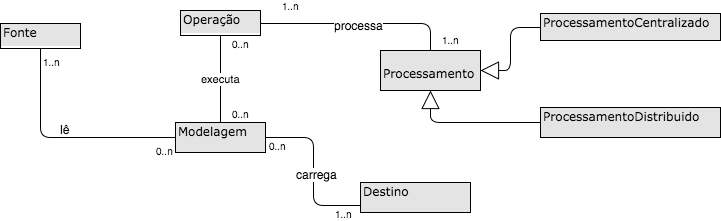
\includegraphics[scale=0.5]{fig/modeloconceitual.png}
	\caption{Modelo conceitual do ETL4NoSQL}
	\label{modeloconceitual}
\end{figure}

\subsubsection{Modelo de Casos de Uso}

Um conjunto de casos de uso pode ser identificado tal como: Ler fonte de dados, Escrever no destino, Modelar dados, Executar operação, Processar operações. O quadro \ref{casosdeuso} mostra a descrição sucinta de cada caso de uso.

\clearpage

\begin{table}[h]
	\centering
	\caption{Modelo de Casos de Uso do ETL4NoSQL}
	\label{casosdeuso}
	\begin{tabular}{|p{14cm}|}
		\hline
			\textbf{Nome:} Ler fonte de dados\\ 
			\textbf{Objetivo:} Fazer a leitura de qualquer tipo de dados a partir de uma fonte de dados.\\ 
			\textbf{Pré-condição:} os parâmetros para permissão de conexão com a fonte de dados devem estar disponíveis.\\ 
			\textbf{Ação:} ler (Fonte)\\ 
		\hline
			\textbf{Nome:} Escrever no destino\\ 
			\textbf{Objetivo:} Fazer a escrita de qualquer tipo de dado a partir do modelo processado pelo ETL4NoSQL em uma base de destino.\\ 
			\textbf{Pré-condição:} os parâmetros para permissão de conexão e escrita com o destino devem estar disponíveis.\\ 
			\textbf{Ação:} escrever (Destino)  \\ 
	\hline
			\textbf{Nome:} Modelar dados\\ 
			\textbf{Objetivo:} Permitir a modelagem dos dados por meio de mecanismos de junção, filtro, união, agregação e outros. \\
			 \textbf{Pré-condição:} os mecanismos de transformação e limpeza devem estar disponíveis para executar a modelagem.\\ 
			 \textbf{Ação:} modelar (Modelagem, Operação)\\ 
	 \hline
	 		\textbf{Nome:} Executar operação\\ 
	 		\textbf{Objetivo:} Armazenar, gerenciar e executar as operações criadas pela ação de modelar.\\
	 		\textbf{Pré-condição:} as operações devem ser criadas previamente pela ação de modelar.\\ 
	 		\textbf{Ação:} executar (Operação, Processamento)\\ 
	 \hline
	 	\textbf{Nome:} Processar operações\\ 
	 	\textbf{Objetivo:} Processar as operações armazenadas de forma centralizada ou distribuída.\\
	 	\textbf{Pré-condição:} as operações precisam estar disponíveis para o processamento.\\ 
	 	\textbf{Ação:} processar (Processamento, Operação)\\ 
	 \hline
	 
	\end{tabular}
\end{table}

\subsubsection{Modelo Comportamental}

Ao construir o modelo comportamental é possível identificar os conceitos com comportamentos mais relevantes para o negócio, bem como os estados e eventos que disparam transições de estados (\cite{itana:2005}). Dessa forma, o diagrama de estados do ETL4NoSQL é apresentado na figura \ref{diagrama_estado}, nele podemos ver as transições de leitura da fonte, validação e identificação dos dados, assim como o tratamento caso os dados não possam ser identificados, subsequente a isso, o armazenamento dos dados para o processamento, a criação dos processos de ETL, a escolha da forma de processamento, execução das operações, e também o tratamento para operações que não puderem ser executadas, e finalmente, a carga dos dados na base destino seguido de uma mensagem de tratamento caso haja sucesso ou não da execução.

\begin{figure}[h]
	\centering
	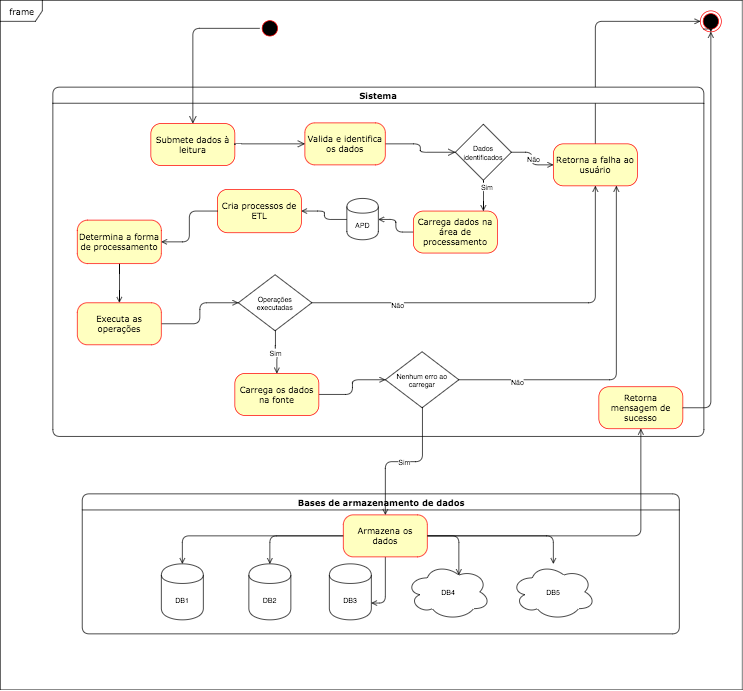
\includegraphics[scale=0.6]{fig/diagrama_estado.png}
	\caption{Diagrama de Estado do ETL4NoSQL}
	\label{diagrama_estado}
\end{figure}

\subsection{Modelagem da Especificação}



\subsubsection{Interfaces de sistema}

\subsubsection{Interfaces de Negócio}

\subsubsection{Especificação da Arquitetura do Componente}

\cite{sommerville:2013}, define o projeto de arquitetura como um processo criativo em que se tenta organizar o sistema de acordo com os requisitos funcionais e não funcionais. Um estilo de arquitetura é um padrão de organização de sistema (\cite{shaw:1996}, \cite{sommerville:2013}), como uma organização cliente-servidor ou uma arquitetura em camadas. Porém, a arquitetura não necessariamente utilizará apenas um estilo, a maioria dos sistemas de médio e grande porte utilizam vários estilos. Para \cite{shaw:1996}, há três questões a serem definidas na escolha do projeto de arquitetura, a primeira é a escolha da estrutura, cliente-servidor ou em camadas, que permita atender melhor aos requisitos. A segunda questão é a respeito da decomposição dos subsistemas em módulos ou em componentes. E por fim, deve-se tomar a decisão de sobre como a execução dos subsistemas é controlada. A descrição da arquitetura pode ser representada graficamente utilizando modelos informais e notações como a UML (\cite{clements:2002}, \cite{sommerville:2013}).


\subsection{Interação entre Componentes}

\subsubsection{Operações da interface de negócio}


\subsection{Especificação de Componentes}



%De forma a detalhar a modelagem de especificação dos componentes deste trabalho, criamos um \textit{workflow} que é apresentado na figura \ref{modeloespecificacao} utilizando modelos informais e notações como a UML (\cite{clements:2002}).

%O modelo de processo do funcionamento da ferramenta ETL4NoSQL, baseado nas notações da UML 2.0 (\cite{clements:2002}), é representado na figura \ref{modeloprocesso}. Esse modelo descreve o processamento dos dados nas atividades de identificação dos dados, obtenção das informações para a importação e o mapeamento dos dados para os esquemas desejados, e também, a atividade dos processos de ETL para por fim dar carga dos dados em DWs, repositórios analíticos ou em arquivos XML.


% fluxo de processos da ferramenta ETL4NoSQL é o diagrama de atividades, que de acordo com a UML 2.0 tem como objetivo mostrar o fluxo de atividades em um único processo. O diagrama mostra como um atividade depende uma da outra. Na figura \ref{diagramaatividades} o diagrama mostra a interação dos componentes ao executar um processo de ETL, onde o estágio inicial é a importação dos dados seguido pelo mapeamento, após a obtenção dos dados necessários é possível a execução dos diversos processos de ETL em uma área de processamento para finalmente os dados serem exportados para base de destino.
%% utilizar diagrama de fluxo de dados para descrever os requisitos do sistema e diagrama de interações


%%construir um diagrama de atividades da execução de um processo de ETL



\section{Componentes do ETL4NoSQL}

A engenharia de software baseada em componentes é uma abordagem fundamentada em reuso para desenvolvimento de sistemas de software, ela envolve o processo de definição, implementação e integração ou composição de componentes independentes não firmemente acoplados ao sistema. Os componentes são independentes, ou seja, não interferem na operação uns dos outros e se comunicam por meio de interfaces bem definidas, os detalhes de implementação são ocultados, de forma que as alterações de implementação não afetam o restante do sistema (\cite{sommerville:2013}). Segundo \cite{sametinger:1997}, componentes são uma parte do sistema de software que podem ser identificados e reutilizados, onde descrevem ou executam funções específicas e possuem interfaces claras, documentação apropriada e a possibilidade de reuso bem definida. Ainda de acordo com o autor, um componente deve ser autocontido, identificável, funcional, possuir uma interface, ser documentado e ter uma condição de reuso. 

De acordo com os requisitos do ETL4NoSQL, foi possível identificar quatro importantes funcionalidades que podem ser definidas como componentes do sistema, a funcionalidade de importação, mapeamento de dados, mecanismos de ETL e o controlador de operações. Os componentes do ETL4NoSQL e suas características são apresentados nas seções seguintes, seguindo as características de componentes adotadas por \cite{heineman:2001}.

%%adicionar modelo de dados e modelo de fluxo de dados

\subsection{Componente de Importação}

Um dos objetivos do framework ETL4NoSQL é possibilitar a integração de várias estruturas de dados, relacionais ou não relacionais, presentes nos sistemas modernos. Para isso, a ferramenta deve permitir a leitura e escrita dos diversos SGBDs existentes que aplicam essas estruturas. A solução encontrada para isso foi desenvolver um componente programável que possibilite a importação dos dados por meio de inserção de parâmetros em linha de comando. Este componente, por ser criado utilizando o paradigma de orientação a objetos, permite também sua extensão, por meio de especialização, para que atenda a especificidade de cada cenário. As características do componente são apresentadas a seguir.

\begin{itemize}
	\item[a)] Interface: Componente responsável pela importação dos dados da base origem.
	
	\item[b)] Nomeação: Import.
	
	\item[c)] Metadados: Este componente contém as informações da base origem como a linguagem de manipulação de dados e meios para estabelecer a conexão com a base, requer uma interação com a interface para o usuário disponibilizar as informações e fornece os dados importados para outros componentes.
	
	\item[d)] Interoperabilidade: Oferece comunicação com outros componentes por meio dos métodos listAll e userData.
	
	%\item[e)] Composição: 
	
	
	\item[e)] Customização: Este componente permite customizar as formas de apresentar os dados importados, de acordo com a necessidade de cada sistema.
	
	\item[f)] Suporte a evolução: Possibilita o suporte aos métodos de acordo com as mudanças de conexões e manipulações de bases de dados futuras.
	
	\item[g)] Empacotamento e utilização: Os métodos são encapsulados e podem  ser utilizados pela importação de sua classe e a interface com o usuário é por meio de linha de comando.
	
\end{itemize}

\subsection{Componente de Mapeamento}

Para viabilizar a organização dos dados em vários tipos de esquemas desejáveis pelo usuário o ETL4NoSQL oferece o componente de mapeamento. Este componente permite definir o esquema dos dados de acordo com a necessidade da aplicação almejada pelo usuário. Por meio de parâmetros de inserção em linha de comando é possível utilizar os esquemas de dados pré-definidos pelo componente, mas também, por utilizar o paradigma de orientação a objetos e as características de reusabilidade dos componentes, é possível especializar e customizar os esquemas conforme a conveniência do usuário.

\begin{itemize}
	\item[a)] Interface: Componente responsável por gerar o mapeamento dos dados oferecidos pelo componente de importação para um esquema relacional.
	
	\item[b)] Nomeação: Map.
	
	\item[c)] Metadados: Este componente requer os dados de uma base de dados para efetuar o mapeamento.
	
	\item[d)] Interoperabilidade: Oferece comunicação com outros componentes por meio dos métodos importData e listMap.
	
	%\item[e)] Composição:
	
	
	\item[e)] Customização: É possível customizar as regras de mapeamento para outros esquemas de dados.
	
	\item[f)] Suporte a evolução: Possibilita o suporte aos métodos de acordo com a necessidade de alterar os esquemas dos dados.
	
	\item[g)] Empacotamento e utilização: Os métodos são encapsulados e podem  ser utilizados pela importação de sua classe e a interface com o usuário é por meio de linha de comando.
	
\end{itemize}


\subsection{Componente de Mecanismos de ETL}

O ETL4NoSQL é um framework de ETL que possibilita a integração de várias estruturas de dados, por isso ele deve apresentar mecanismos que viabilizem as principais operações de ETL conhecidas pela literatura. Dessa forma, para disponibilizar as operações de ETL, o ETL4NoSQL possui um componente de mecanismos de ETL que permite executar processos de ETL como extração, limpeza/transformação e carga de dados. Além das operações básicas de ETL, o componente permite a especialização e criação de mecanismos permitindo a customização das operações de ETL conforme a necessidade do usuário.

\begin{itemize}
	\item[a)] Interface: Componente que contém métodos que realizam as principais operações de ETL presentes na literatura. 
	
	\item[b)] Nomeação: MechanismETL.
	
	\item[c)] Metadados: Este componente requer dados de controle para realizar as operações por meio de seus métodos.
	
	\item[d)] Interoperabilidade: Oferece comunicação com outros componentes por meio dos métodos exec e process.
	
	%\item[e)] Composição:
	
	
	\item[e)] Customização: É possível customizar e criar mecanismos de acordo com a necessidade de cada processo de ETL.
	
	\item[f)] Suporte a evolução: Deve possibilitar o suporte aos métodos de acordo com a necessidade de alterar os esquemas dos dados.
	
	\item[g)] Empacotamento e utilização: Os métodos deverão ser encapsulados e poderão ser utilizados pela importação de sua classe e a interface com o usuário será por meio de linha de comando.
	
\end{itemize}

\subsection{Componente de Operações}

Para proporcionar o controle dos processos de ETL executados pelo framework, o ETL4NoSQL possui o componente de operações. Este componente é responsável pelo controle das operações dos processos de ETL, ele assegura a execução dos mecanismos de ETL de acordo com a necessidade do usuário. É possível também, customizar e especializar as operações deste componente.

\begin{itemize}
	\item[a)] Interface: Componente responsável por criar e executar processos de ETL.
	
	\item[b)] Nomeação: Componente de Operação.
	
	\item[c)] Metadados: Este componente deverá possibilitar a comunicação com o componente de mecanismos de ETL e deverá criar e executar processos de ETL.
	
	\item[d)] Interoperabilidade: Deve possibilitar a comunicação entre outros componentes.
	
	%\item[e)] Composição:
	
	
	\item[e)] Customização: É possível customizar os processos de ETL criados.
	
	\item[f)] Suporte a evolução: Deve possibilitar o suporte aos métodos de acordo com a necessidade de alterar os processos.
	
	\item[g)] Empacotamento e utilização: Os métodos deverão ser encapsulados e poderão ser utilizados pela importação de sua classe e a interface com o usuário será por meio de linha de comando.
	
\end{itemize}

\section{Considerações Finais}
